\section{Etude des besoins}

The LAB.E.S project seeks to provide an innovative platform for real-time monitoring of laboratory operations. This solution will concentrate automated data and offer it to the management team in a clear, structured format. It also aims to automate all administrative papers and handle all laboratory operations.

\subsection{Identification des besoins fonctionnels}
\begin{enumerate}
    \item

Connection to PLCs: To retrieve equipment data in real time, the platform must be able to connect to the laboratory's PLCs.
\item
Continuous supervision: This must allow for continuous tracking of laboratory activities and test results.
\item
Test Subject Sheet Management: Employees must be able to generate and manage test subject sheets directly from the platform.
\item
Data display: Collected data should be freely available and visible on laboratory screens.
\item
A dashboard should pull together all of the collected data, providing management with a clear, unifying picture.
\item
Intuitive User Interface: To make data access and interpretation easier, the platform must have a user-friendly, intuitive, and simple interface.
\item
Data confidentiality and integrity must be ensured by strong security measures.
\end{enumerate}
\subsection{Étude des besoins non fonctionnels}

\begin{enumerate}
\item

Performance: The platform must react swiftly to queries while remaining highly available.

\item
Reliability: It must be resilient, with fail-safe procedures and maximum uptime.

\item
Scalability: The platform must be capable of handling an increase in workload, particularly by including additional test benches and PLCs.

\item
Security:
Security mechanisms must be in place to prevent unwanted access and maintain data integrity.

\item
Compatibility: The platform must be interoperable with various PLC kinds as well as current laboratory systems.

\item
Maintainability: The platform should be simple to manage, with frequent upgrades and enough technical assistance.

\item
Usability: The platform should be simple to use, with an intuitive UI and a quick learning curve.

\item
Portability: It must be flexible to multiple hardware and software infrastructures.
\end{enumerate}

%\subsection{Backlog du produit}
\subsection{Identification des users}
\begin{description}\item[Admin:]\end{description}  The administrator's responsibility is to have broad access and control over the LABES platform. He or she is in charge of overall system administration, which includes configuration, security, and user management.

\begin{description} \item[Pilote de Sujet:]\end{description}  The subject manager is responsible for supervising and coordinating specialized laboratory operations related to a given test subjects and projects.


\subsection{Use case {\&} Validation Case}
Use Cases define the specific interactions between users and the system. They specify the actions that users may take on the site.
Validation Cases are required to guarantee that each Use Case performs as expected. They contain verification processes to ensure that functionality fulfills the specifications and is properly implemented.
\begin{figure}[H]
    \centering
    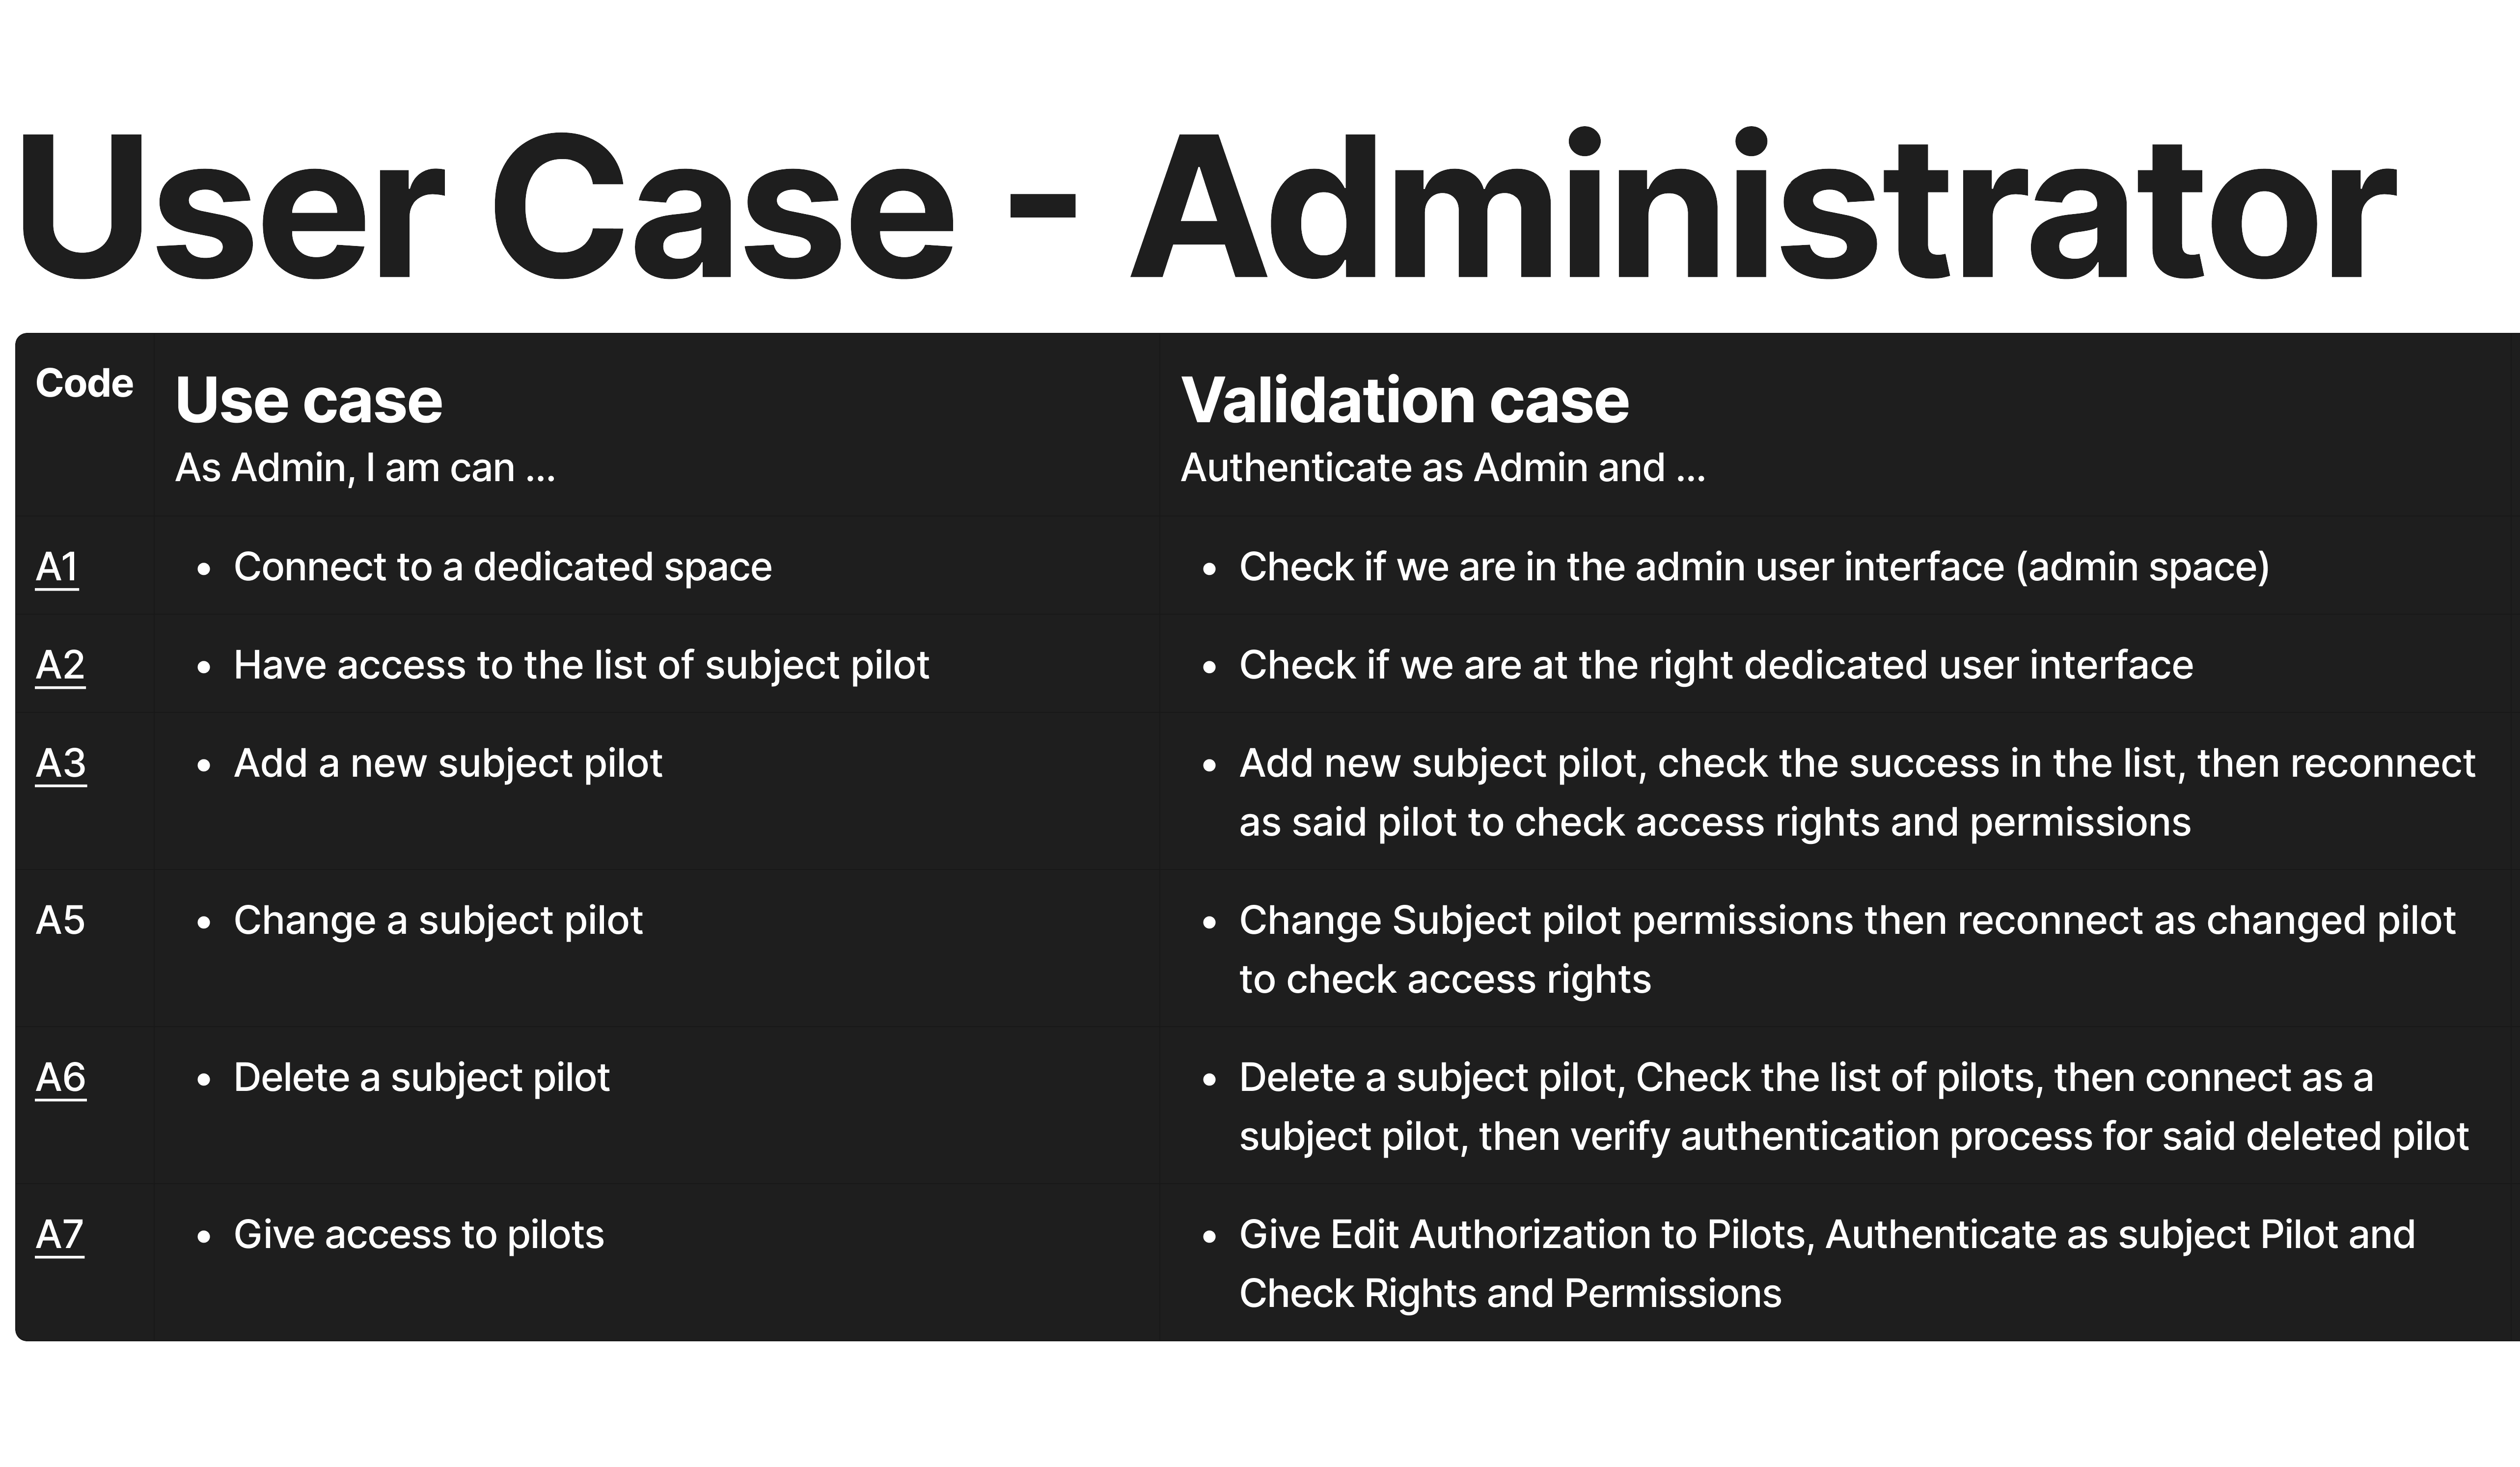
\includegraphics[width=1.1\textwidth]{chapters/2/img/use case.png}
    \caption{Use Case}
    \label{fig:campus}
\end{figure}
\begin{figure}[H]
    \centering
    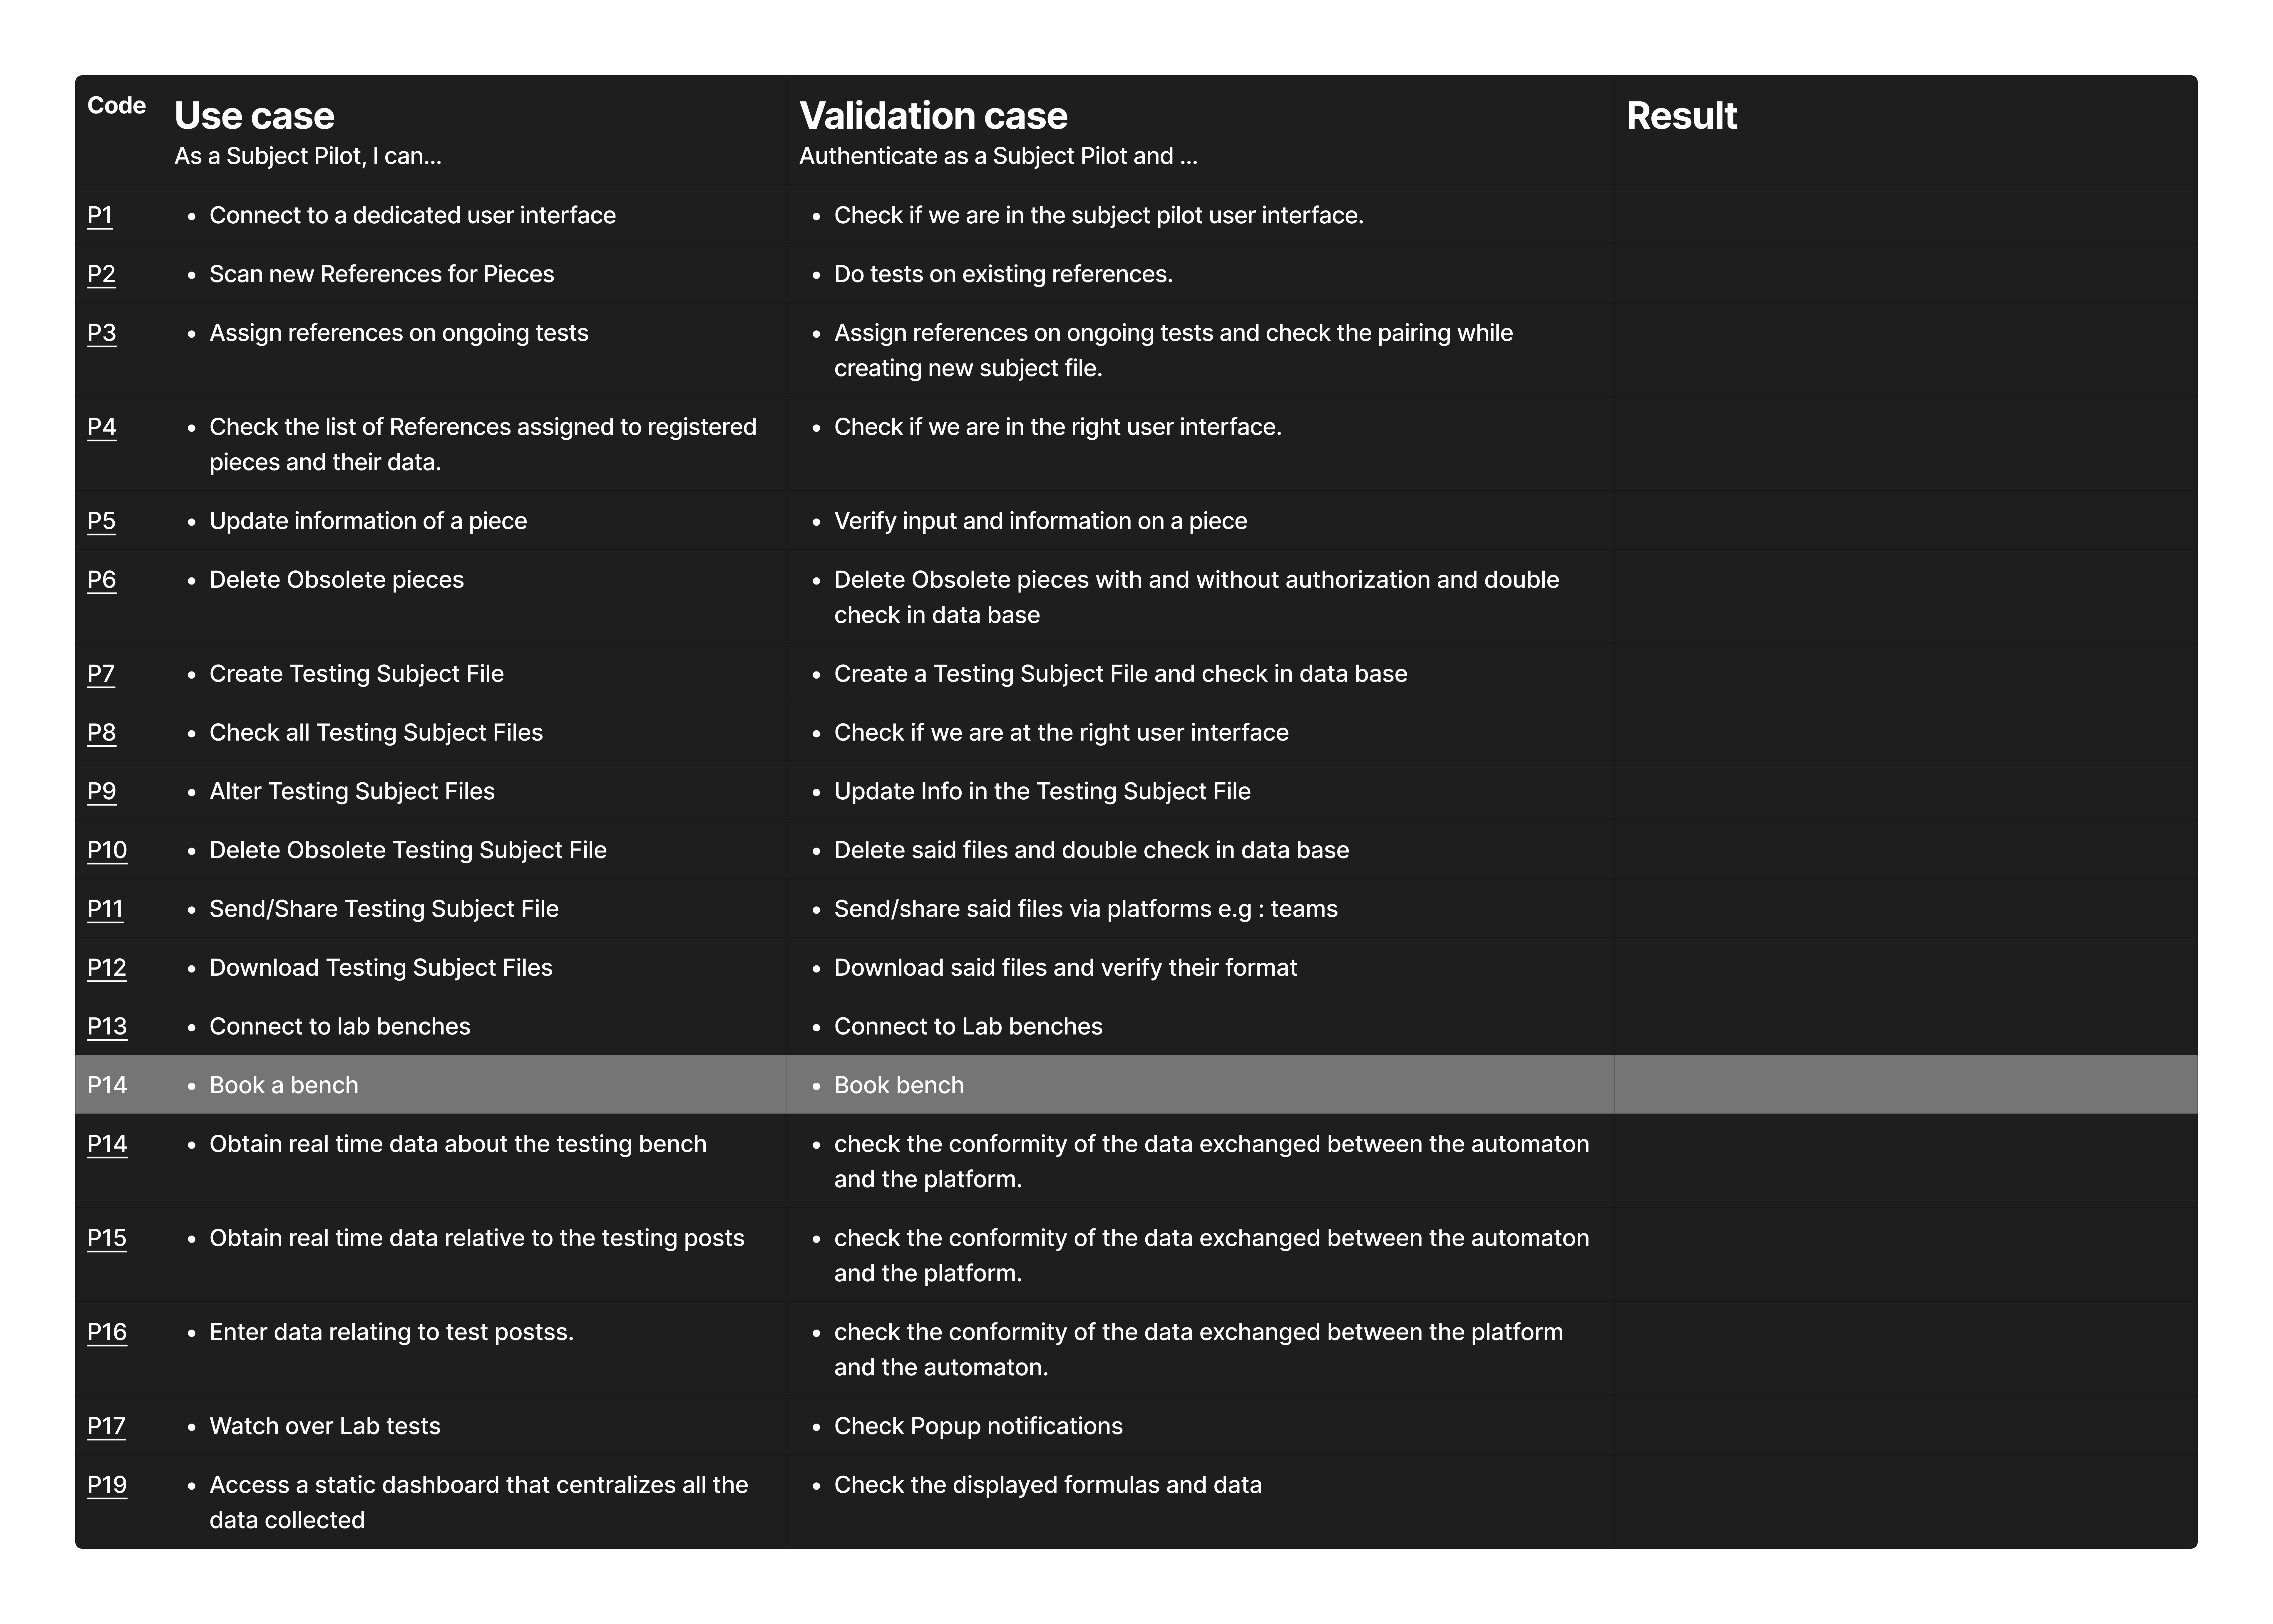
\includegraphics[width=1.\textwidth]{chapters/2/img/1.png}
    \caption{Use Case}
    \label{fig:campus}
\end{figure}

\subsection{User Flow}
A User Flow is a graphic representation of the steps a user takes to achieve a given objective on the platform. It specifies all of the processes, interactions, and decisions that the user must make to complete an action.


\subsubsection {Utilité des User Flow}

\begin{description} \item[Compréhension du parcours utilisateur :]\end{description} 
Understanding the user journey: User flows assist in visualizing and comprehending the path that the user travels through the interface, hence identifying possible friction points.
\begin{description} \item[Amélioration de l'expérience utilisateur :]\end{description} 
Designers can enhance the experience by mapping user flows and making use of each stage.
\begin{description} \item[Communication claire :]\end{description} 
User flows serve as a guide for developers, designers, and other clients, ensuring that everyone understands how users will interact with the system.
\begin{description} \item[Identification des besoins fonctionnels :]\end{description} 
They help specify the functionality needed at each stage of the user experience, ensuring that the application satisfies user expectations.

\subsubsection {Composants d'un User Flow}

\begin{description}\item[Administrateur:]\end{description} 
\begin{itemize}
  \item Entry points: These are the pages where users start their journey, such as the home or login page.
  \item Steps: Each interaction or action taken by the user, such as clicking a button or completing a form.
  \item Decisions: The different options or pathways open to the user, such as whether to register or log in.
  \item Exit points: The points at which the user achieves his goal or quits the journey, such as when logging out.
\end{itemize}
\begin{figure}[H]
    \centering
    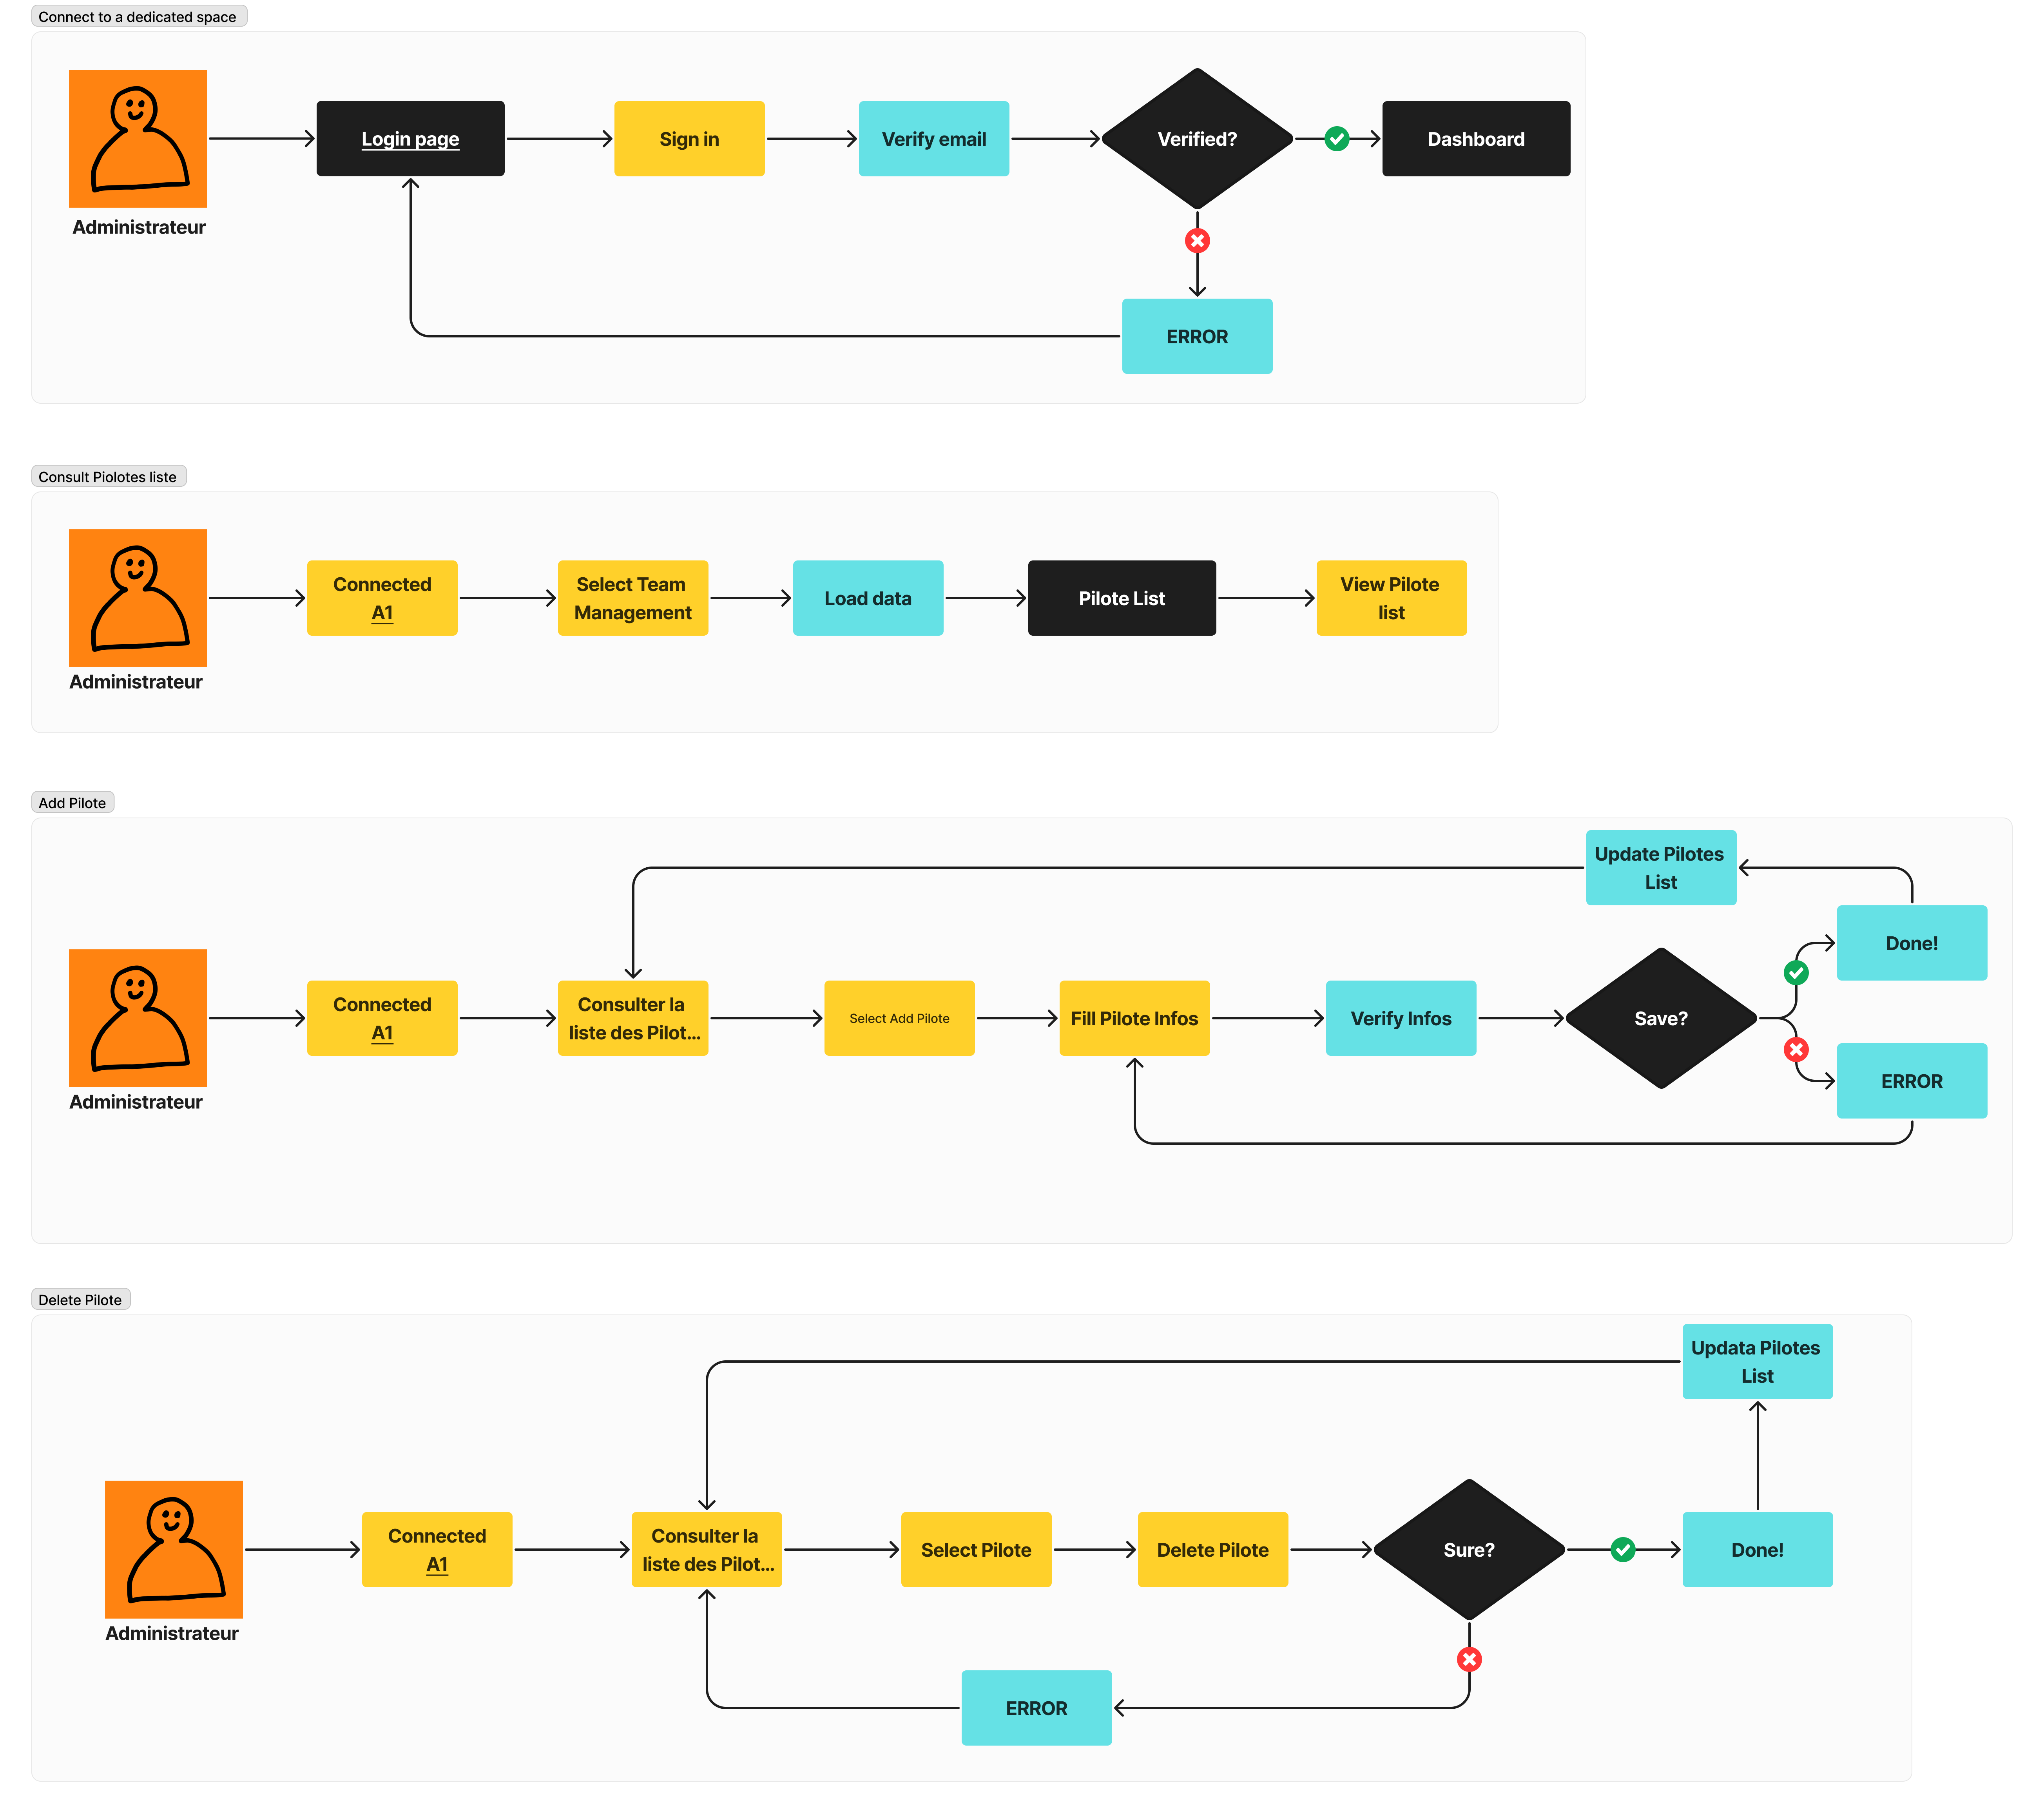
\includegraphics[width=1\textwidth]{chapters/2/img/2.png}
    \caption{Use Case}
    \label{fig:campus}
\end{figure}


\begin{figure}[H]
    \centering
    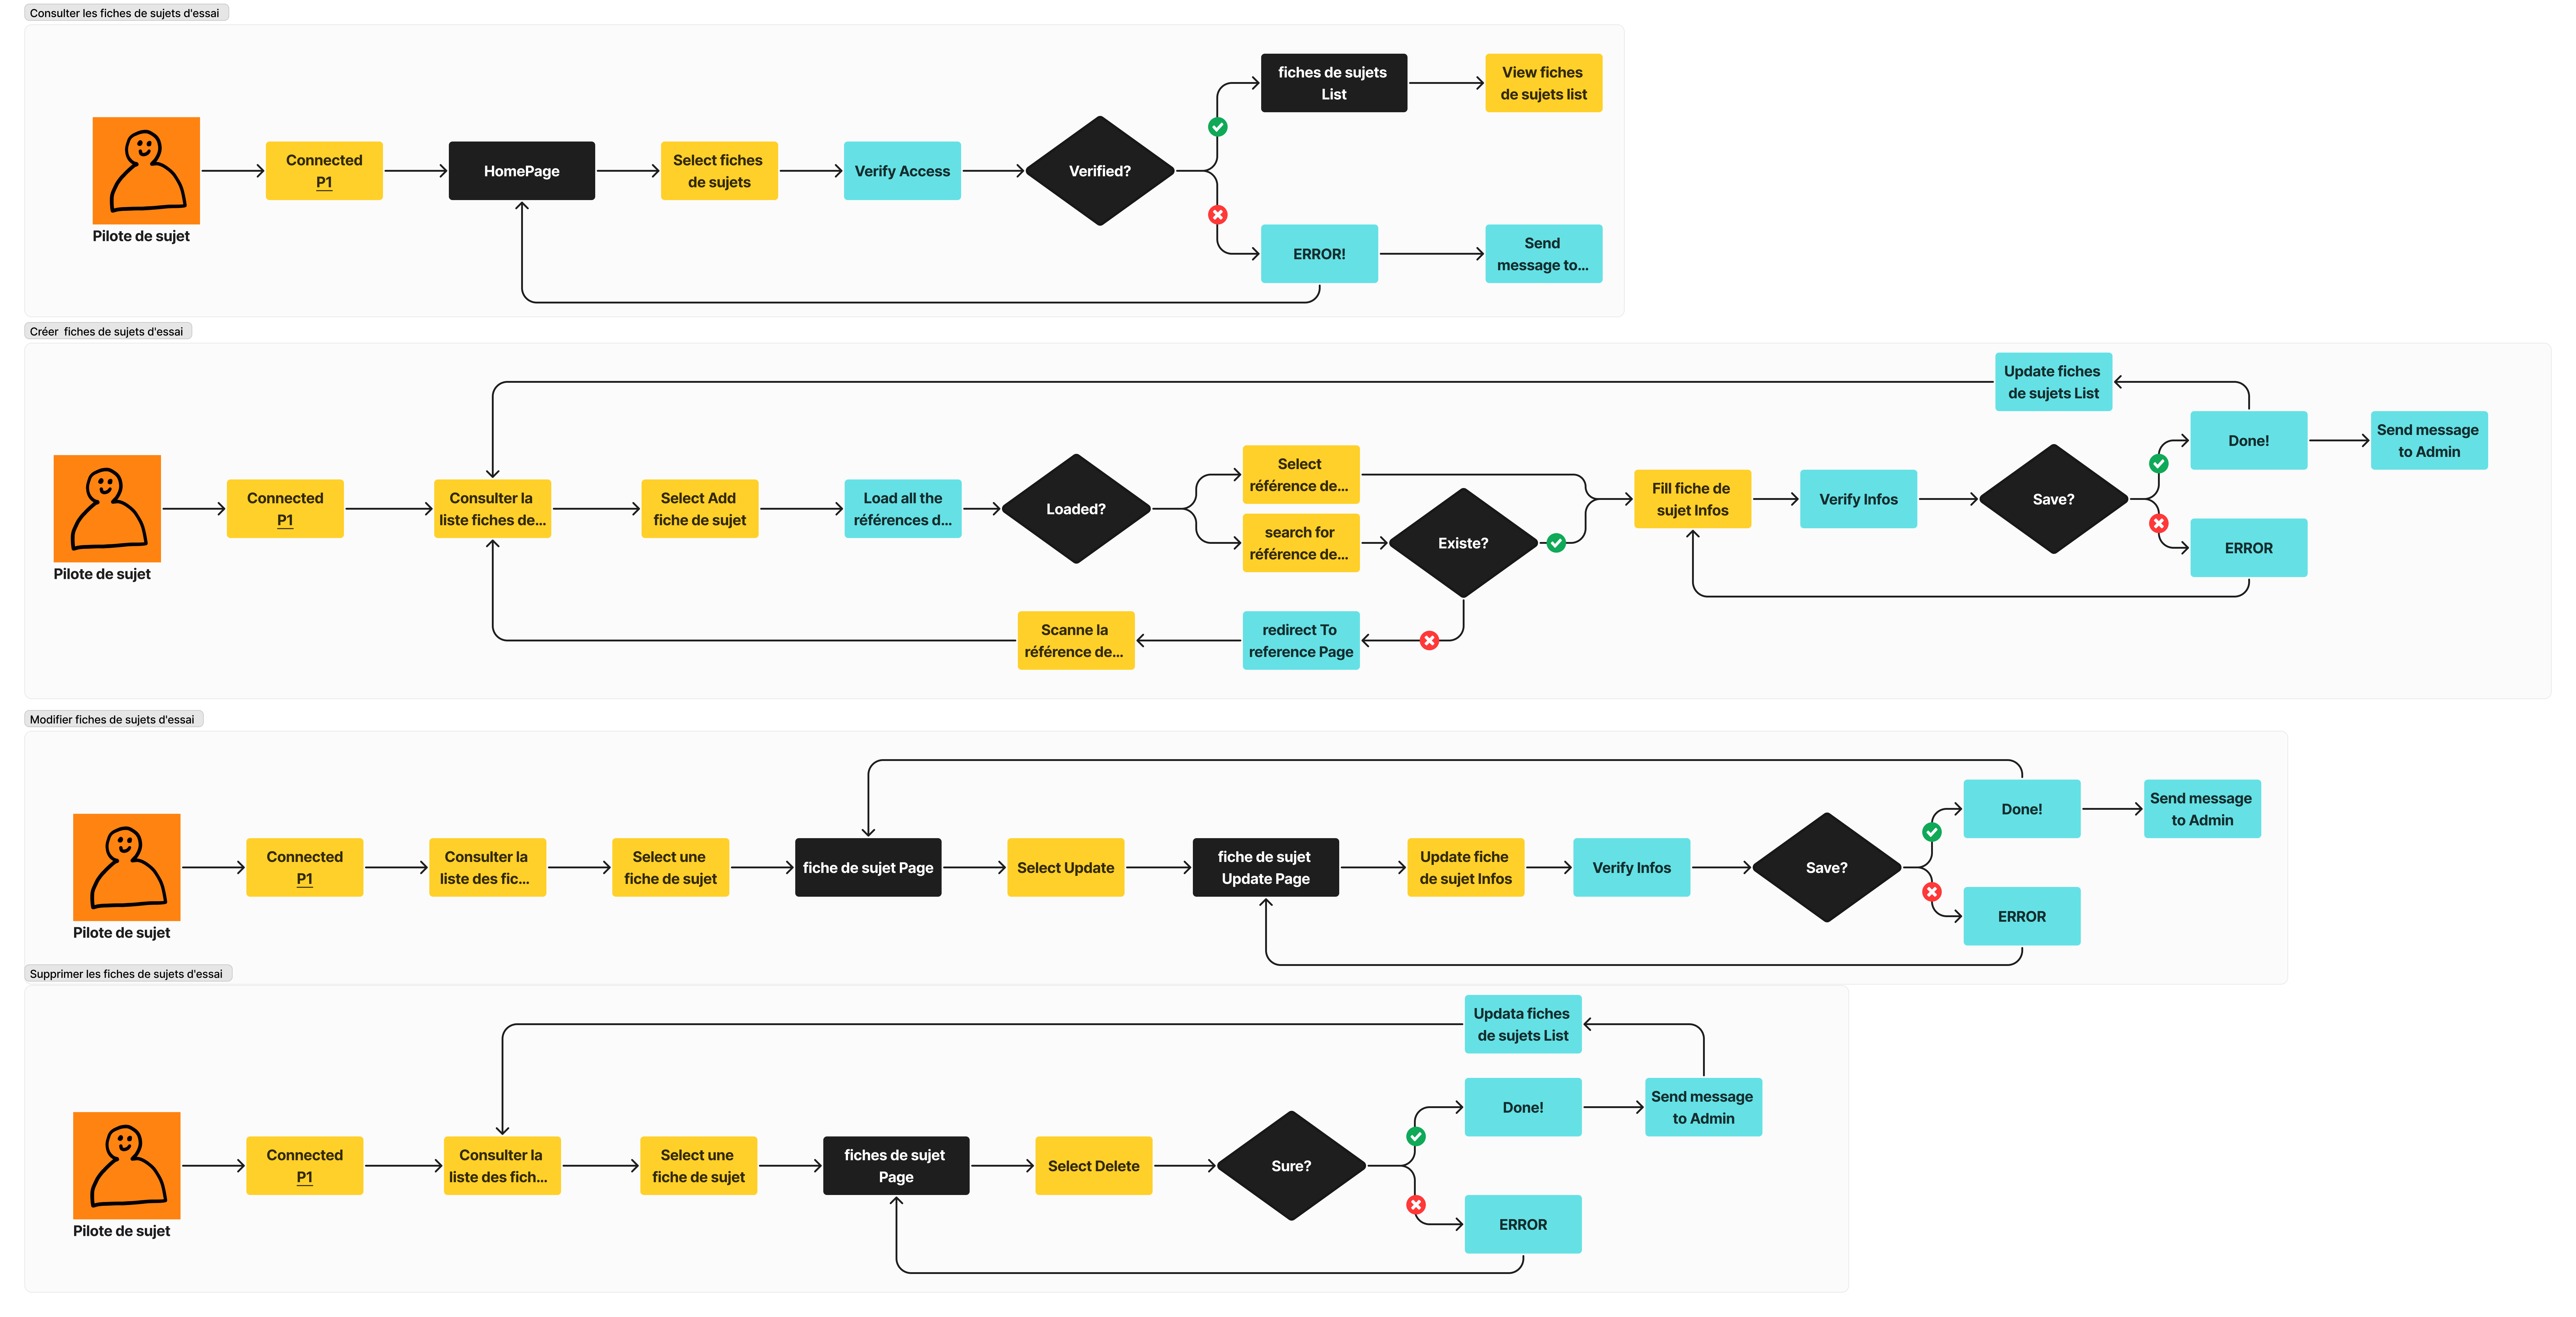
\includegraphics[width=1.5\textwidth, angle=90]{chapters/2/img/3.png}
    \caption{Use Case}
    \label{fig:campus}
\end{figure}
\begin{figure}[H]
    \centering
    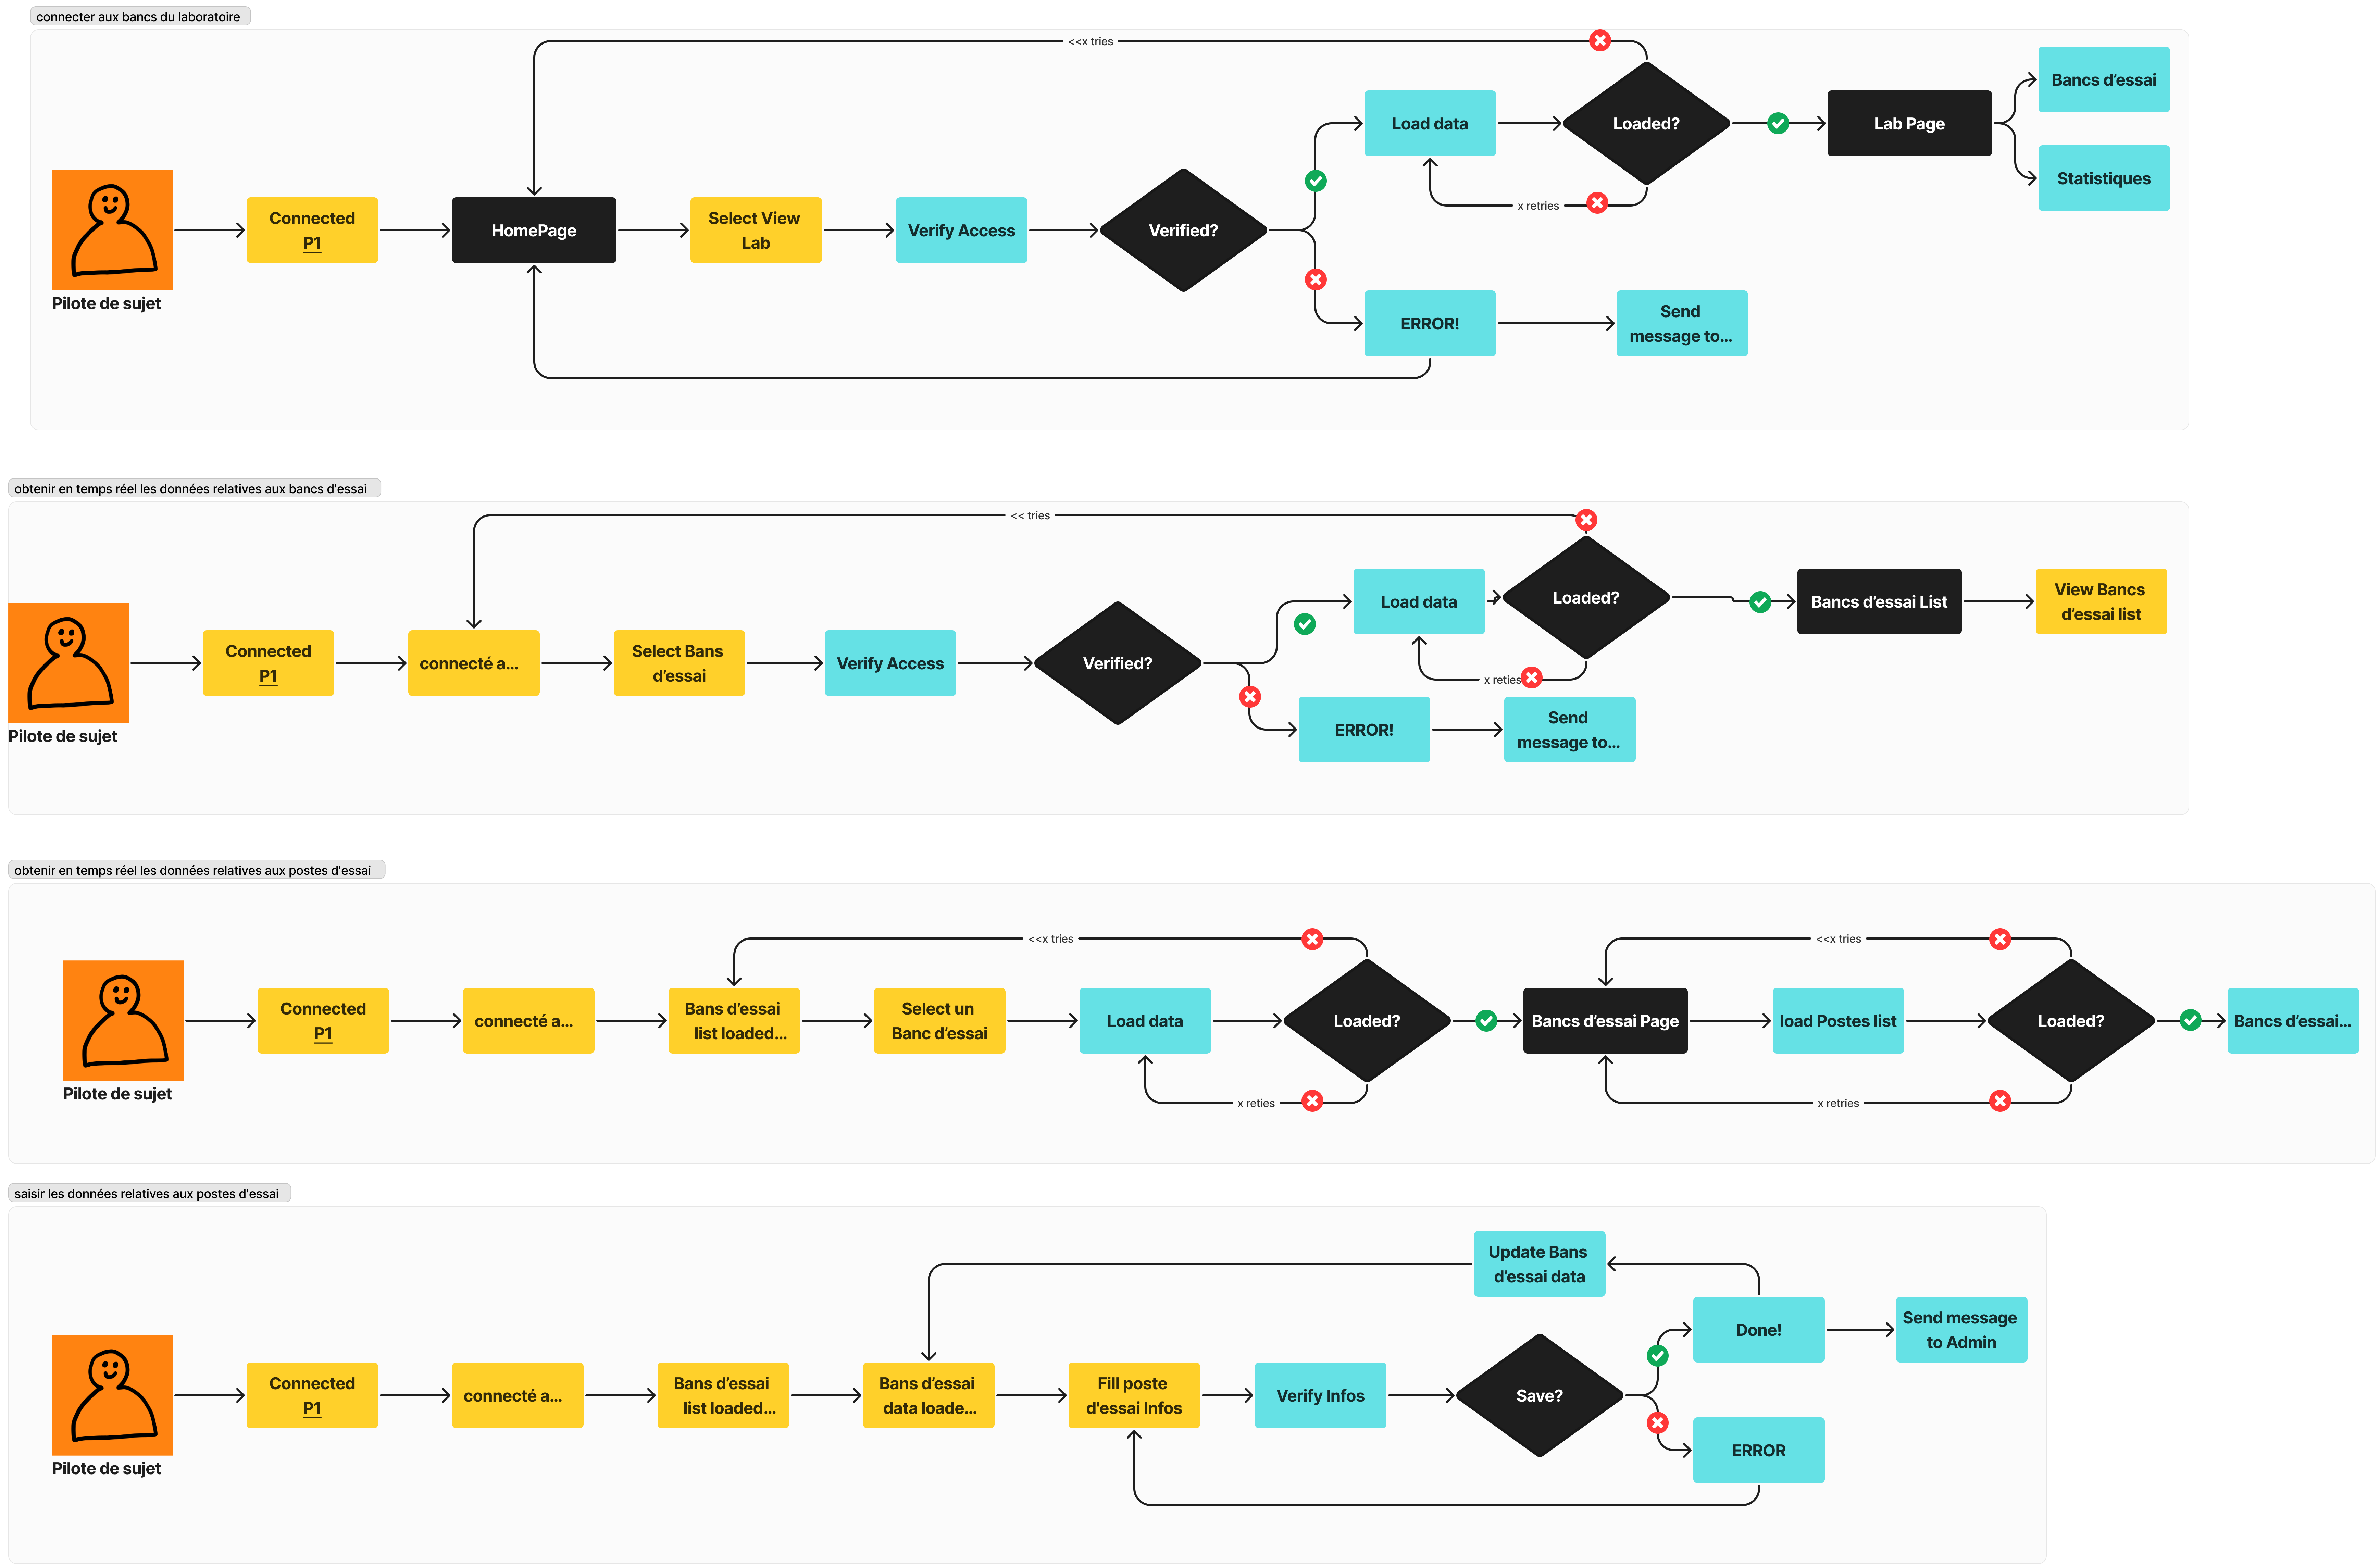
\includegraphics[width=1.5\textwidth, angle=90]{chapters/2/img/4.png}
    \caption{Use Case}
    \label{fig:campus}
\end{figure}
%(par exemple, confirmation d'achat, déconnexion).
\end